% DL4STG PA3 report body — include from main.tex
% Code: \url{https://github.com/ttqureshi/DL4STG-PA3}

\section{What Does a Sum Remember? (Q1)}

In message passing on a graph, a node $v$ pools messages from its neighbours $\mathcal{N}(v)$ (excluding $v$ itself), then applies a readout:
\begin{equation}
  h_v = \rho\!\left(\sum_{u \in \mathcal{N}(v)} \phi(x_u)\right).
\end{equation}
Here each neighbour reports a trend $x_u \in \{-1,0,+1\}$, $\phi$ encodes the message, and $\rho$ is any nonlinearity applied \emph{after} aggregation---as in a GCN without degree normalization.

\subsection{Affine messages}

If $\phi(x) = wx + c$, then
\[
  \sum_{u \in \mathcal{N}(v)} \phi(x_u)
  = w \sum_{u \in \mathcal{N}(v)} x_u + |\mathcal{N}(v)|\,c
  = w S_v + n_v c,
\]
with $n_v = |\mathcal{N}(v)|$ and $S_v = \sum_{u \in \mathcal{N}(v)} x_u$.
The scalar fed to $\rho$ depends only on $(n_v, S_v)$.
Two neighbourhoods with the same counts and sum of trends look identical to the layer, even when the split between steady, slowing, and speeding neighbours differs.

Example: both neighbourhoods have $n_v=5$ and $S_v=0$, but A has trends $(-1,-1,0,+1,+1)$ (one steady neighbour) while B has $(-1,0,0,0,+1)$ (three steady neighbours).
For every $w,c$, $\sum_u \phi(x_u) = 5c$, so $h_v = \rho(5c)$ in both cases.
Nonlinearity after the sum cannot recover how many neighbours were steady.

\subsection{Nonlinear scalar encoding}

When $1 \le n_v \le K$, we can use mixed-radix constants $\phi(-1)=1$, $\phi(0)=\beta$, $\phi(+1)=\beta^2$ with $\beta = K+1$.
The encoded sum $n_- + \beta n_0 + \beta^2 n_+$ uniquely determines the counts $(n_-, n_0, n_+)$ because $\beta > K$ prevents carries between digits.
Recovery is by modulo and floor operations on that sum.
We need $\beta > K$; smaller bases would map different count triples to the same aggregate.

A simpler target is the count of \emph{non-steady} neighbours: $\phi(-1)=\phi(+1)=1$, $\phi(0)=0$, so the sum equals $n_- + n_+$.

\subsection{One-hot messages: sum, mean, and max}

Fix $\phi(-1)=(1,0,0)$, $\phi(0)=(0,1,0)$, $\phi(+1)=(0,0,1)$.
Let $(n_-, n_0, n_+)$ be trend counts and $\mathbf{m}$ the aggregated vector.
\textbf{Sum} gives $\mathbf{m} = (n_-, n_0, n_+)$.
\textbf{Mean} gives $(n_-/n_v,\, n_0/n_v,\, n_+/n_v)$.
\textbf{Max} gives $(\mathbb{1}[n_->0],\,\mathbb{1}[n_0>0],\,\mathbb{1}[n_+>0])$.

\begin{itemize}
  \item \textbf{Count steady neighbours:} only \textbf{sum} works ($n_0 = m_2$). Mean and max collide on examples with the same proportions but different $n_0$.
  \item \textbf{More than half slowing:} \textbf{sum} and \textbf{mean} work ($m_1>0.5$ for mean). \textbf{Max} fails: e.g.\ $(-1,-1,-1,0,0)$ vs.\ $(-1,-1,0,+1,+1)$ both give $(1,1,1)$ but only the first has a slowing majority.
  \item \textbf{Any neighbour slowing:} sum, mean, and max all work (for mean/max, the first coordinate is positive iff $n_->0$).
\end{itemize}

Takeaway: aggregation is a lossy bottleneck unless messages are rich enough or the aggregator keeps sufficient statistics (counts, not just pooled ratios).

\section{Which Way Is the Slowdown Moving? (Q2)}

Forty ring sensors $i = 0,\ldots,39$ with wrap-around.
True backward motion of a slowdown pattern is $x_i(t+1) = x_{i+1}(t)$ (one step: \texttt{np.roll}$(x,-1)$).

\subsection{Symmetric neighbour layer}

The symmetric update
\[
  \hat{x}_i(t+1) = a\, x_i(t) + b\,\big(x_{i-1}(t) + x_{i+1}(t)\big)
\]
treats left and right neighbours equally.
For an isolated spike at sensor 20, the true one-step shift puts mass only on sensor 19; SSE $=a^2+(b-1)^2+b^2$ minimizes at $a=0$, $b=\tfrac{1}{2}$: the symmetric layer splits mass to both neighbours and cannot copy a one-sided shift.

On a Gaussian bump rolled for 20 steps, truth translates the peak one sensor per step against traffic with nearly fixed shape.
The symmetric layer diffuses energy to both sides, smearing the bump (Figure~\ref{fig:q2-heatmaps}).

\begin{figure}[t]
  \centering
  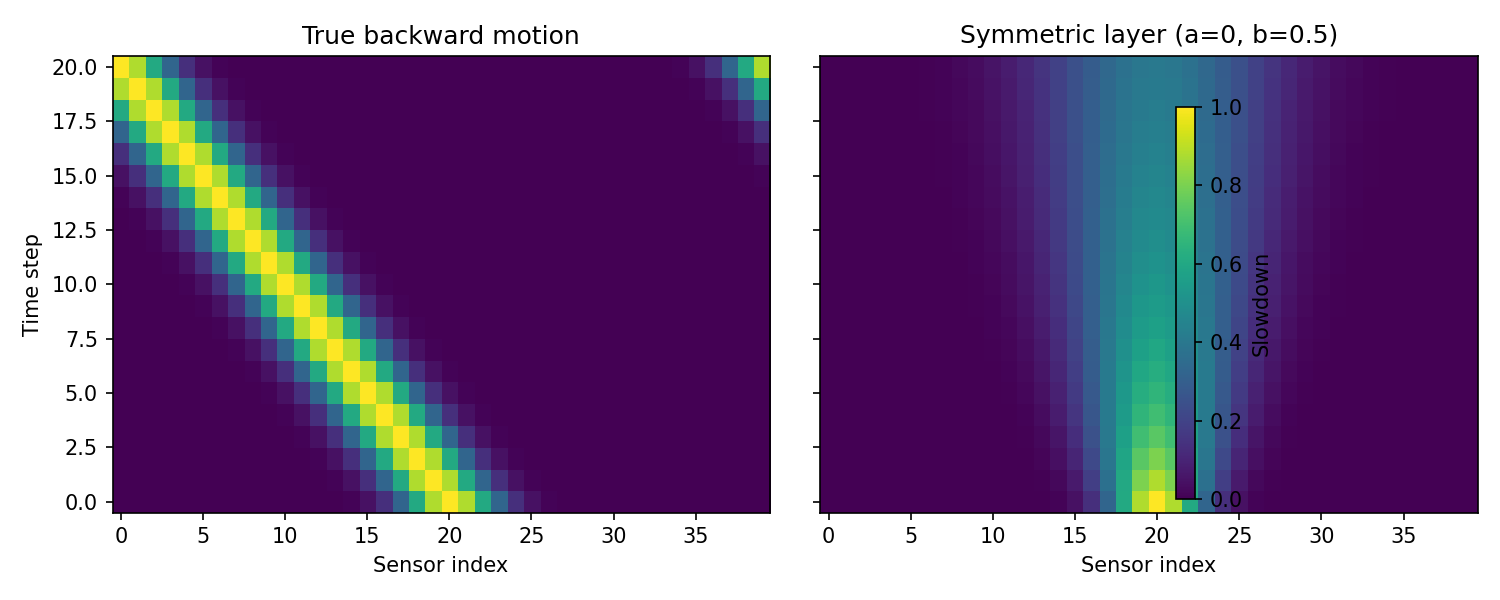
\includegraphics[width=\linewidth]{../figures/q2a_bump_heatmaps.png}
  \caption{Q2(a): true backward rollout vs.\ symmetric neighbour layer on a ring bump (sensor index horizontal, time vertical).}
  \label{fig:q2-heatmaps}
\end{figure}

Equal weights on $x_{i-1}$ and $x_{i+1}$ cannot represent directed transport: the shift operator is antisymmetric in the two neighbours, but the layer only sees their symmetric part.

\subsection{Directional weights}

\[
  \hat{x}_i(t+1) = a\, x_i(t) + w_{-}\, x_{i-1}(t) + w_{+}\, x_{i+1}(t)
\]
with $a=0$, $w_{-}=0$, $w_{+}=1$ gives $\hat{x}_i = x_{i+1}$, matching backward motion exactly.
As a 1D kernel on $[x_{i-1}, x_i, x_{i+1}]$, $\mathbf{k} = [0, 0, 1]$ with circular padding on the ring.

\subsection{Temporal coefficient with equal spatial weights}

\[
  \hat{x}_i(t+1) = a\, x_i(t) + b\,\big(x_{i-1}(t) + x_{i+1}(t)\big) + c\, x_i(t-1).
\]
Under backward flow, $x_i(t-1) = x_{i-1}(t)$; choosing $a=0$, $b=1$, $c=-1$ cancels the wrong symmetric part:
\[
  \hat{x}_i(t+1) = x_{i-1}(t) + x_{i+1}(t) - x_{i-1}(t) = x_{i+1}(t).
\]
Under forward flow $x_i(t+1)=x_{i-1}(t)$, the same coefficients still work because then $x_i(t-1)=x_{i+1}(t)$.
History breaks directional ambiguity: $x_i(t-1)$ ties the current spatial pattern to \emph{how} the field evolved, even when $b$ weights both neighbours equally.

\section{Dataset and Graph Construction (Q3)}

We use LargeST San Diego (District 11): $N=716$ PeMS sensors, aligned with the CA road-network adjacency via \texttt{sd\_meta.csv} ID2 indexing.
Implementation and scripts live in the course repository\footnote{\url{https://github.com/ttqureshi/DL4STG-PA3}}.

\subsection{Data extraction and resampling}

PeMS flow from 5-minute bins in \texttt{ca\_his\_raw\_2020.h5} and \texttt{ca\_his\_raw\_2021.h5} is resampled to 15-minute steps.
Following LargeST, we take the \textbf{mean} of the three 5-minute counts in each window and round to integers.
Before \texttt{fillna(0)}: 2,542,017 NaN cells (5.06\% of the tensor; all 716 sensors affected). Imputation: zero fill (LargeST).
Real flow built from Kaggle HDF5 via \texttt{scripts/fetch\_real\_flow\_g.py}; shape $[70176, 716]$.
Output tensor $X \in \mathbb{R}^{T \times 716}$ is stored with train-split metadata for windowing.

\begin{figure}[t]
  \centering
  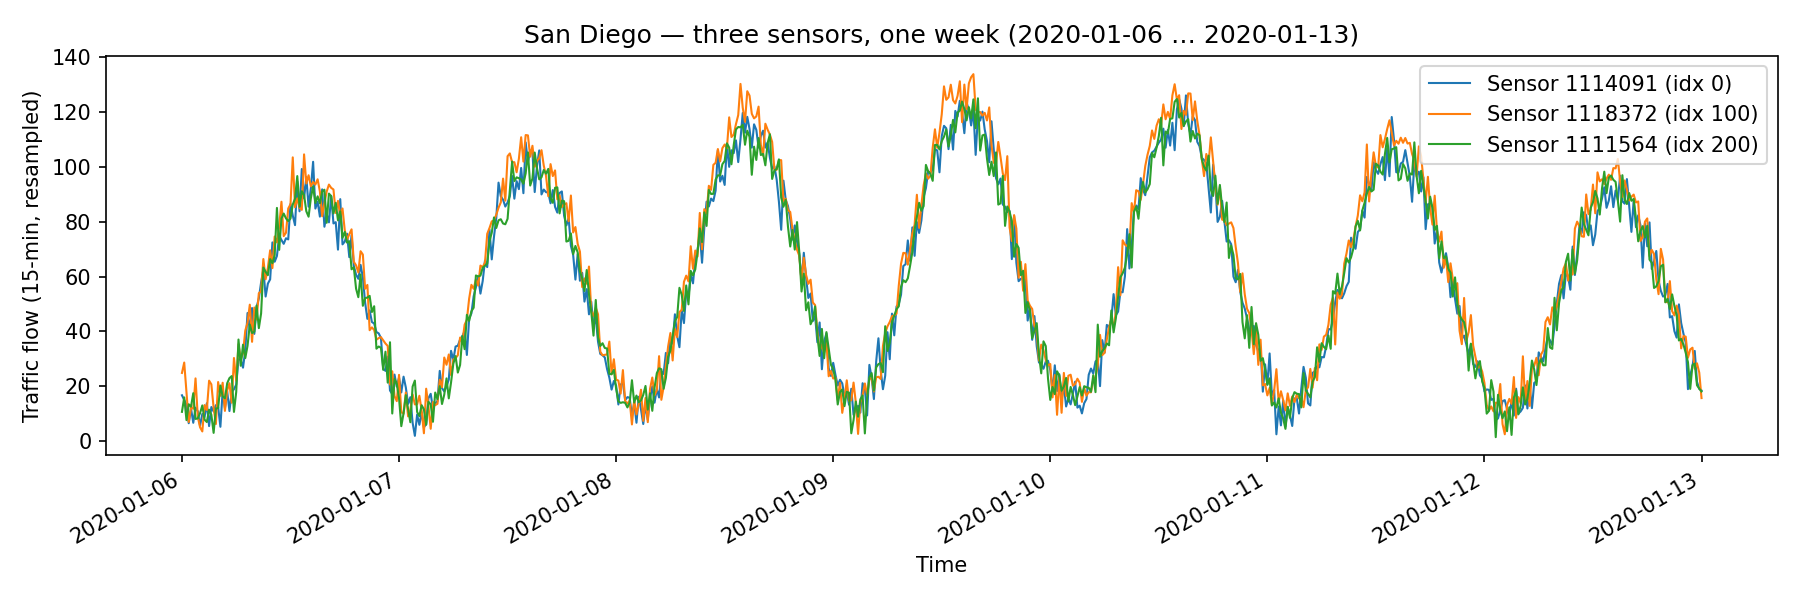
\includegraphics[width=\linewidth]{../figures/q3/q3a_three_sensors_one_week.png}
  \caption{Three SD sensors, one week (2020-01-06 to 2020-01-13; indices 0, 100, 200).}
  \label{fig:q3-timeseries}
\end{figure}

\subsection{Traffic graph $A$}

We extract the SD submatrix $A_{\mathrm{SD}} = A_{\mathrm{CA}}[I,I]$ from \texttt{ca\_rn\_adj.npy}.
Off-diagonal $A_{ij} \neq 0$ means sensors $i$ and $j$ are linked on the road network in LargeST (distance-based adjacency), not merely close in space.

On this build: $716$ nodes, \textbf{17,319} directed off-diagonal nonzeros, mean degree $\approx 24.19$, sparsity $\approx 3.38\%$; the SD submatrix is not exactly symmetric (LargeST distances).

\begin{figure}[t]
  \centering
  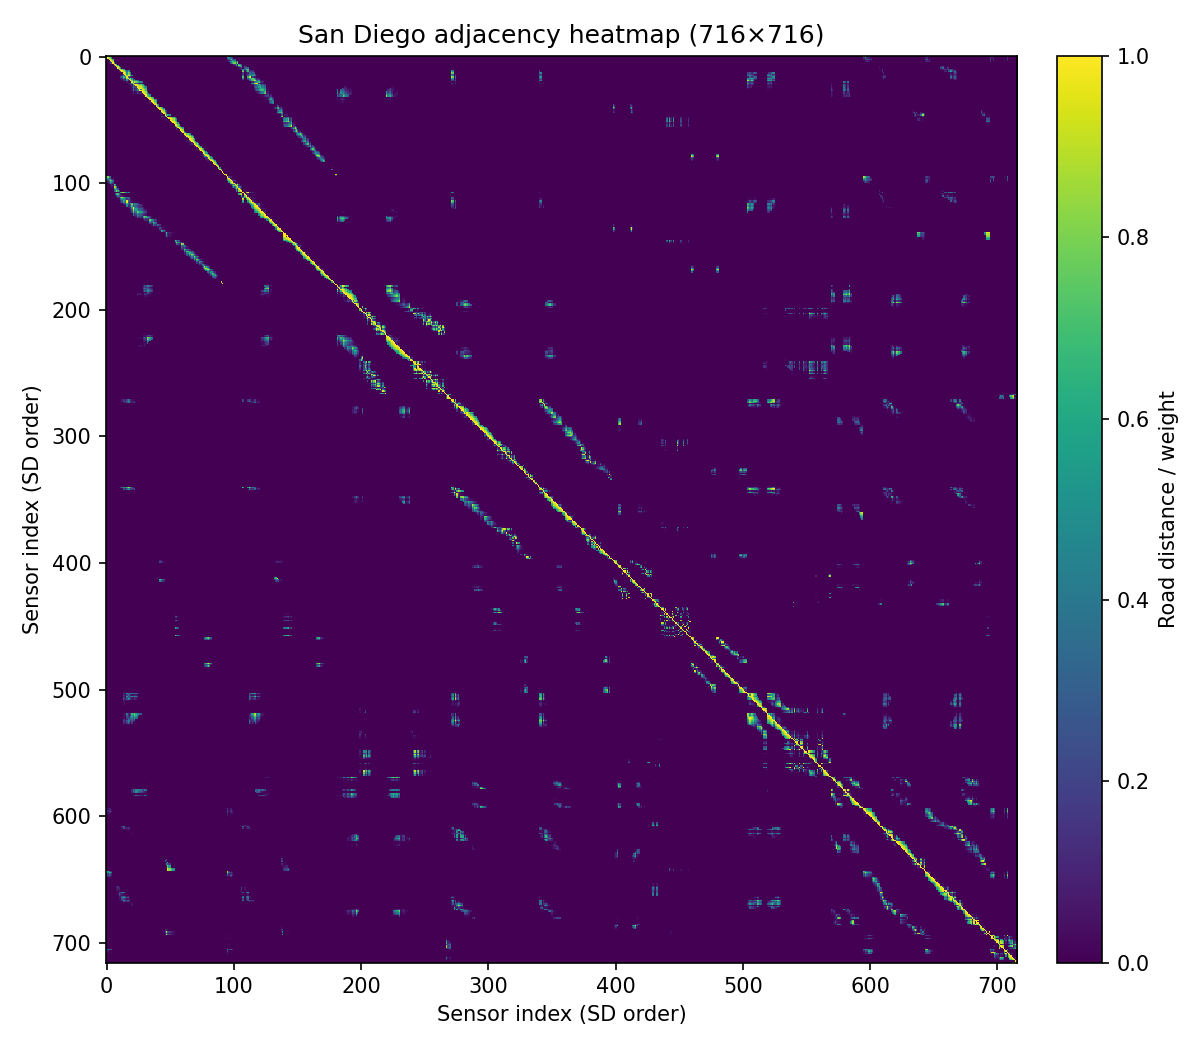
\includegraphics[width=0.48\linewidth]{../figures/q3/q3b_adjacency_heatmap.png}
  \hfill
  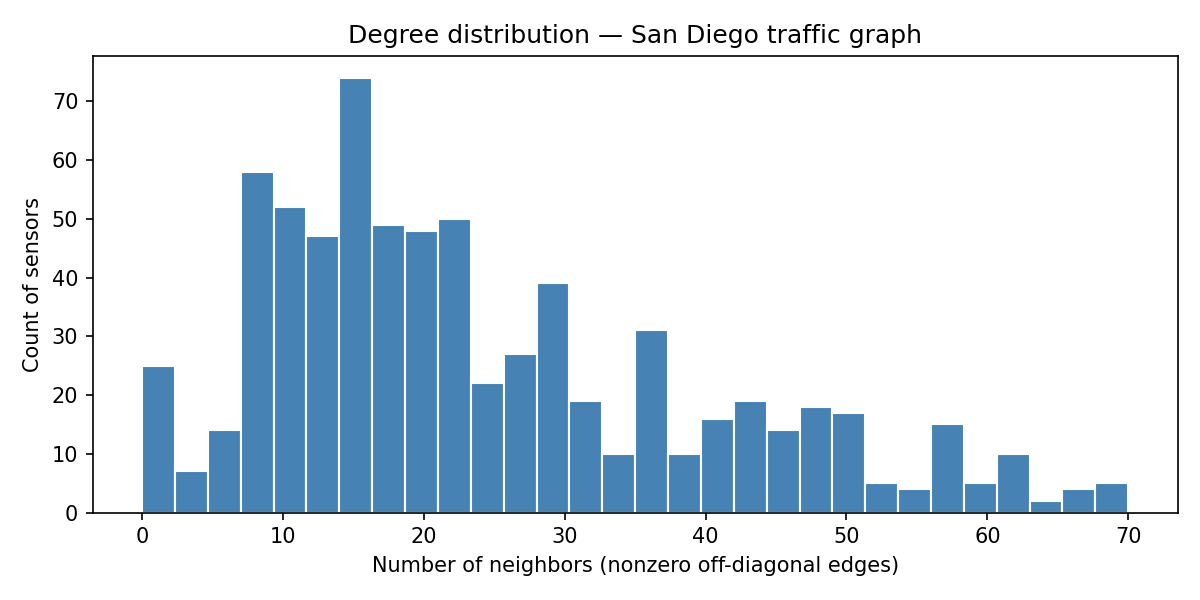
\includegraphics[width=0.48\linewidth]{../figures/q3/q3b_degree_distribution.png}
  \caption{SD adjacency heatmap (cropped for display) and degree distribution.}
  \label{fig:q3-graph}
\end{figure}

\subsection{Neighbourhoods}

Example sensor index 0 (ID 1114091): 23 one-hop and 23 two-hop neighbours (\texttt{q3c\_neighborhood\_example.json}).

One-hop neighbours are $\mathcal{N}_1(i) = \{ j : A_{ij} \neq 0 \}$.
Two-hop nodes are reachable within two edges, excluding $i$ and one-hop nodes.
Neighbours help because congestion and demand propagate along corridors; upstream sensors often lead the target.
One-hop message passing is local; two-hop widens the receptive field but can mix distant, weakly related sensors.
Stacking many graph layers risks over-smoothing and diluting temporal detail---especially on a sparse graph where most signal is local.

\section{Spatio-Temporal Forecasting Setup (Q4)}

We forecast 15-minute flow on $G=(V,E)$, $|V|=716$.
Raw adjacency $A$ encodes network links; message passing uses the normalized operator with self-loops:
\begin{equation}
  \hat{A} = D^{-1/2}(A + I)\,D^{-1/2}, \qquad D_{ii} = \sum_j (A+I)_{ij}.
\end{equation}

\subsection{Windows, splits, and normalization}

Input horizon $T_{\mathrm{in}}=8$, prediction horizon $H=4$.
For end time $t$, the model sees past flows $x_i(t - T_{\mathrm{in}} + 1 + \tau)$ and predicts $x_i(t+h)$ for $h=1,\ldots,H$.
Windows stay inside each split: train on calendar 2020, validate on 2021 Q1, test on 2021 Q2--Q4.
Global train mean $\mu$ and std $\sigma$ normalize all splits; metrics are computed after denormalization.

\subsection{ST-GNN encoder}

Each sensor history passes through 1D convolutions along time and pooling to $z_i \in \mathbb{R}^{d}$, $d=32$.
One graph layer aggregates neighbour embeddings:
\begin{equation}
  H = \mathrm{ReLU}\!\left(\hat{A}\, Z\, W_g\right),
\end{equation}
i.e.\ row $i$ of $\hat{A}Z$ is a weighted sum over $\mathcal{N}(i)\cup\{i\}$.
A shared linear head maps $H$ (or $Z$) to $H$ future steps per node.

\subsection{Temporal-only baseline}

The same temporal encoder and head run \emph{without} graph convolution ($H=Z$).
This isolates whether spatial message passing adds value beyond per-sensor temporal patterns.
Training uses Adam at $10^{-3}$, L1 loss on normalized targets, early stopping on validation MAE, seed 42.

\section{Adjacency Variants (Q5)}

All spatial models share the Q4 temporal block; only $A_{\mathrm{msg}}$ in $H=\mathrm{ReLU}(A_{\mathrm{msg}} Z W_g)$ changes.

\subsection{Fixed road-network adjacency}

$A_{\mathrm{msg}} = \hat{A}$ from Q3.
Self-loops in $A+I$ and symmetric normalization keep message magnitudes stable across high- and low-degree sensors.
The adjacency buffer is fixed during training; only convolution and temporal weights learn.

\subsection{Adaptive (learned) adjacency}

Embeddings $E_1, E_2 \in \mathbb{R}^{N \times d_e}$, $d_e=10$, define
\[
  S = \mathrm{ReLU}(E_1 E_2^\top), \qquad
  (A_{\mathrm{adaptive}})_{ij} = \mathrm{softmax}_j(S_{ij}).
\]
Each row is a distribution over message receivers.
Top-$k$ sparsification ($k=20$) keeps the largest entries per row and renormalizes.
The GCN uses $A_{\mathrm{adaptive}}$ directly (already row-stochastic; no extra $D^{-1/2}$).

\subsection{Hybrid adjacency}

\[
  A_{\mathrm{hybrid}} = \alpha\,\hat{A} + (1-\alpha)\,A_{\mathrm{adaptive}}, \quad \alpha=0.5,
\]
with row normalization after mixing.
$\hat{A}$ anchors propagation to the road map; $A_{\mathrm{adaptive}}$ can add statistical shortcuts between correlated but non-adjacent sensors.

\section{Experimental Comparison (Q6)}

We compare four runs on the 2021 test split (denormalized MAE and RMSE).
Table~\ref{tab:comparison} summarizes results after 20 epochs (seed 42).

\begin{table}[t]
  \centering
  \caption{Test metrics on LargeST SD flow (April--December 2021). Lower is better.}
  \label{tab:comparison}
  \begin{tabular}{llrrrrrr}
    \toprule
    Model & Adj. & Val MAE & Val RMSE & Test MAE & Test RMSE & Time (s) & Seed \\
    \midrule
    temporal\_only & --- & 18.96 & 31.84 & 21.15 & 34.51 & 3163 & 42 \\
    stgnn\_adaptive & adapt. & 22.65 & 41.18 & 26.82 & 45.32 & 3862 & 42 \\
    stgnn\_hybrid & hybrid & 24.49 & 41.83 & 28.16 & 45.19 & 4498 & 42 \\
    stgnn\_fixed & fixed & 53.89 & 86.12 & 60.37 & 94.53 & 3892 & 42 \\
    \bottomrule
  \end{tabular}
\end{table}

\paragraph{Interpretation.}
\textbf{No ST-GNN beats the temporal-only baseline} on this split.
Per-sensor temporal convolutions already capture most predictable structure---daily and weekly rhythms, short-term inertia---without mixing neighbours through $A$.

Among graph models, \textbf{adaptive adjacency is best} (MAE 26.82), then hybrid (28.16), then fixed $\hat{A}$ (60.37).
Fixed message passing on the road graph \emph{hurts} badly here.
That gap suggests the LargeST distance adjacency misaligns with how flow errors actually couple across sensors: forcing $\hat{A}$ may inject noise from weak or misleading edges.
Learned $A_{\mathrm{adaptive}}$ is flexible enough to redistribute messages, but not enough to close the gap to temporal-only.

Figure~\ref{fig:q6-preds} shows one-step-ahead predictions on test sensors 0, 100, and 200 for the hybrid run (representative ST-GNN behaviour).

\begin{figure}[t]
  \centering
  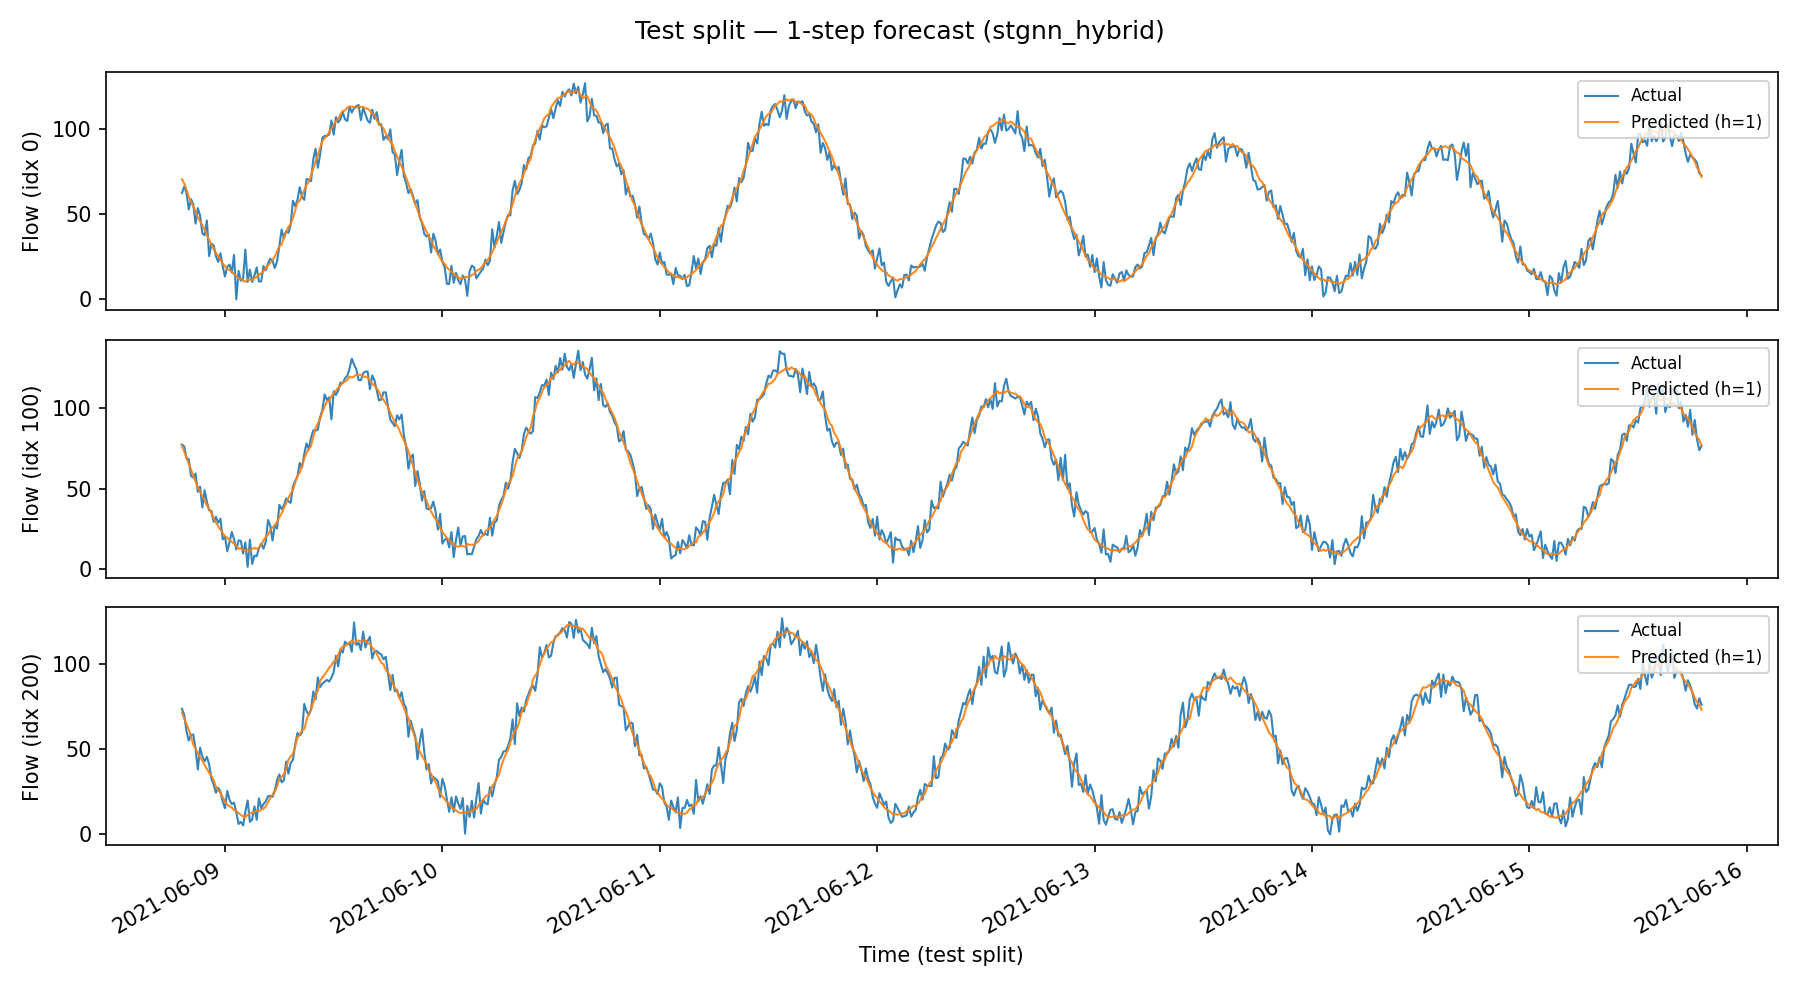
\includegraphics[width=\linewidth]{../figures/q6/predictions_stgnn_hybrid_three_sensors.png}
  \caption{Q6: predicted vs.\ actual flow ($h=1$) on three test sensors (hybrid model).}
  \label{fig:q6-preds}
\end{figure}

Quantitative comparison of learned vs.\ fixed structure (entropy, correlation on edges, top-$k$ overlap) is reported in Section~\ref{sec:q7}.

\section{Analysis of Learned Spatial Structure (Q7)}
\label{sec:q7}

We ask whether $A_{\mathrm{adaptive}}$ rediscovers the road graph or learns a different message topology.

\subsection{Visual comparison}

Figures~\ref{fig:q7-learned}--\ref{fig:q7-diff} crop the first $128 \times 128$ sensors for readability.
$\hat{A}$ is sparse and banded along true network links.
$A_{\mathrm{adaptive}}$ is more diffuse and block-like: the model routes to statistically similar sensors, not only physical neighbours.
The difference map shows where learning strengthens or suppresses edges relative to $\hat{A}$.

\begin{figure}[t]
  \centering
  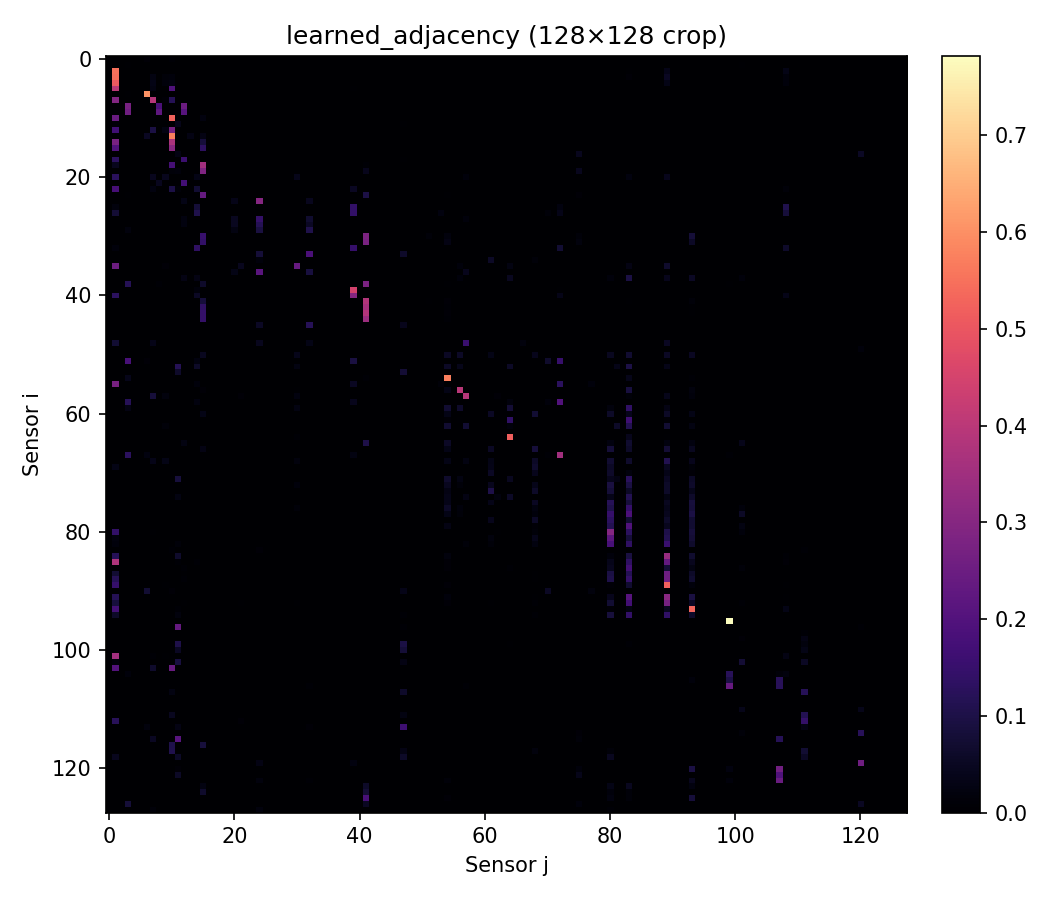
\includegraphics[width=0.32\linewidth]{../figures/q7/stgnn_adaptive_learned_adjacency.png}
  \hfill
  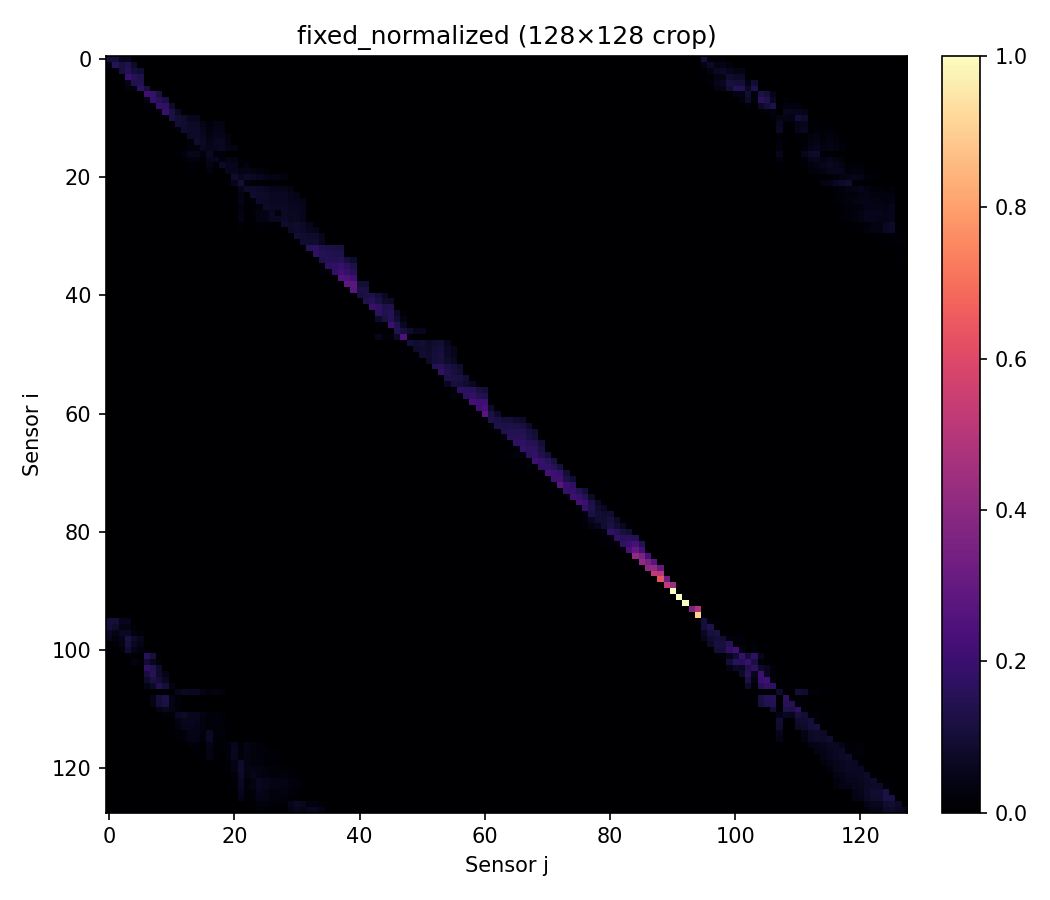
\includegraphics[width=0.32\linewidth]{../figures/q7/stgnn_adaptive_fixed_normalized.png}
  \hfill
  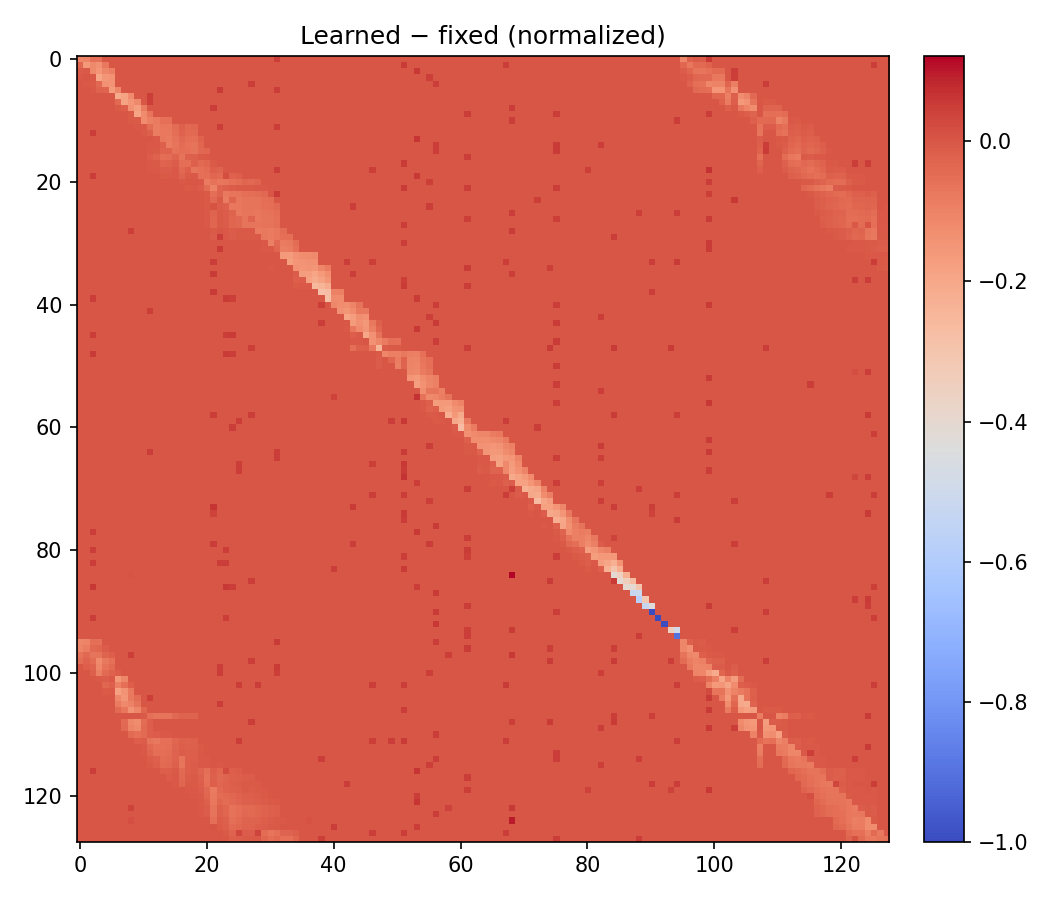
\includegraphics[width=0.32\linewidth]{../figures/q7/stgnn_adaptive_difference.png}
  \caption{Adaptive run: learned $A_{\mathrm{adaptive}}$, fixed $\hat{A}$, and learned minus fixed (crop).}
  \label{fig:q7-learned}
\end{figure}

\begin{figure}[t]
  \centering
  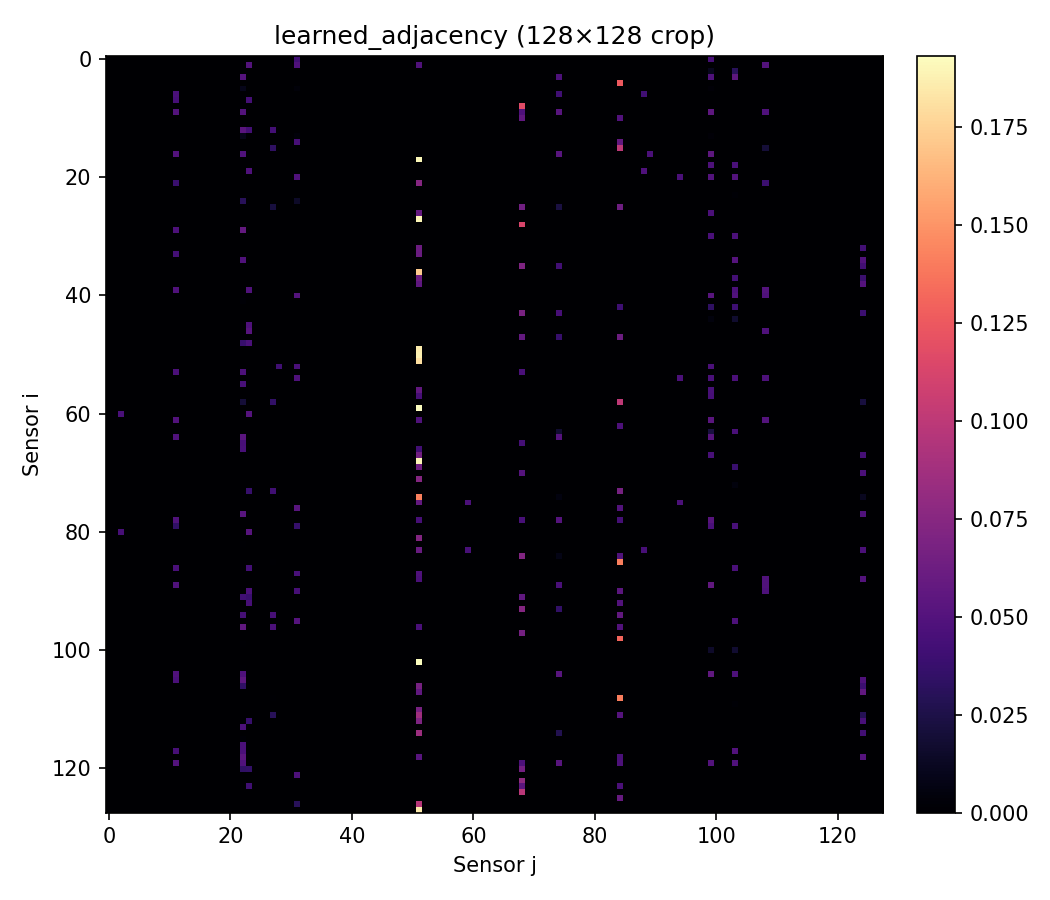
\includegraphics[width=0.32\linewidth]{../figures/q7/stgnn_hybrid_learned_adjacency.png}
  \hfill
  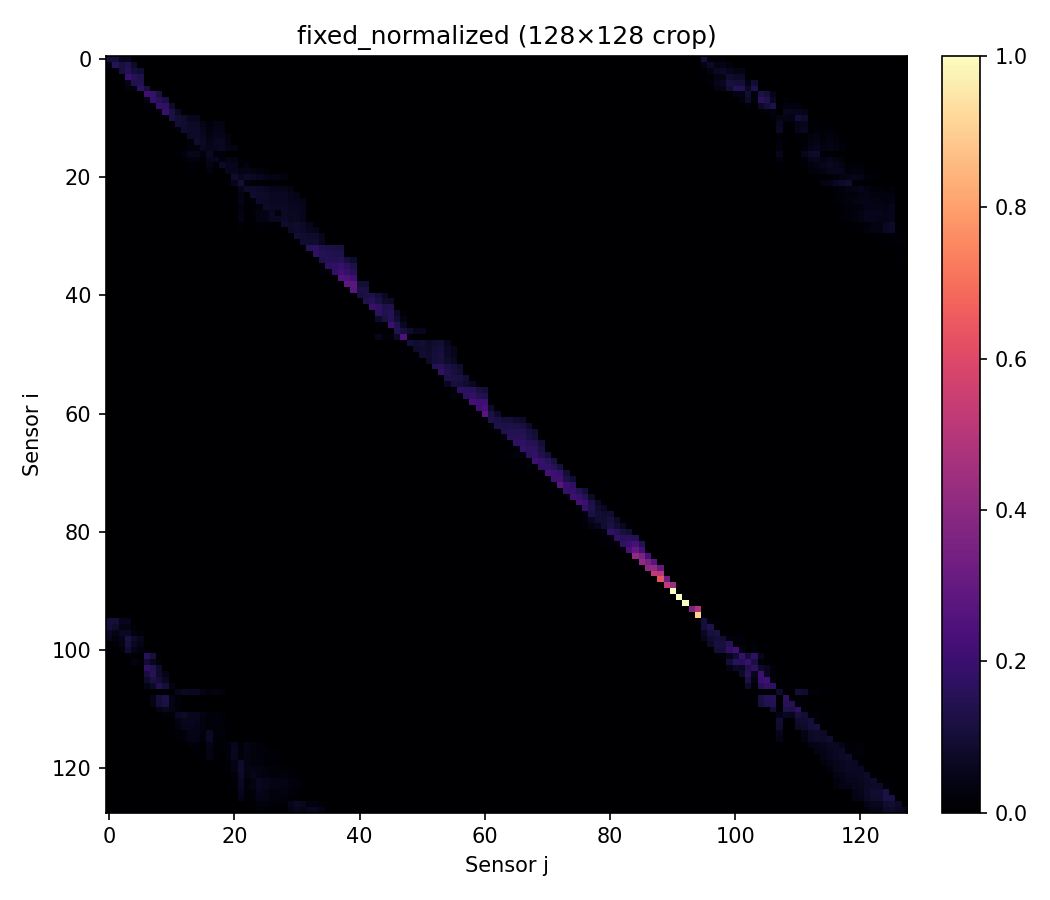
\includegraphics[width=0.32\linewidth]{../figures/q7/stgnn_hybrid_fixed_normalized.png}
  \hfill
  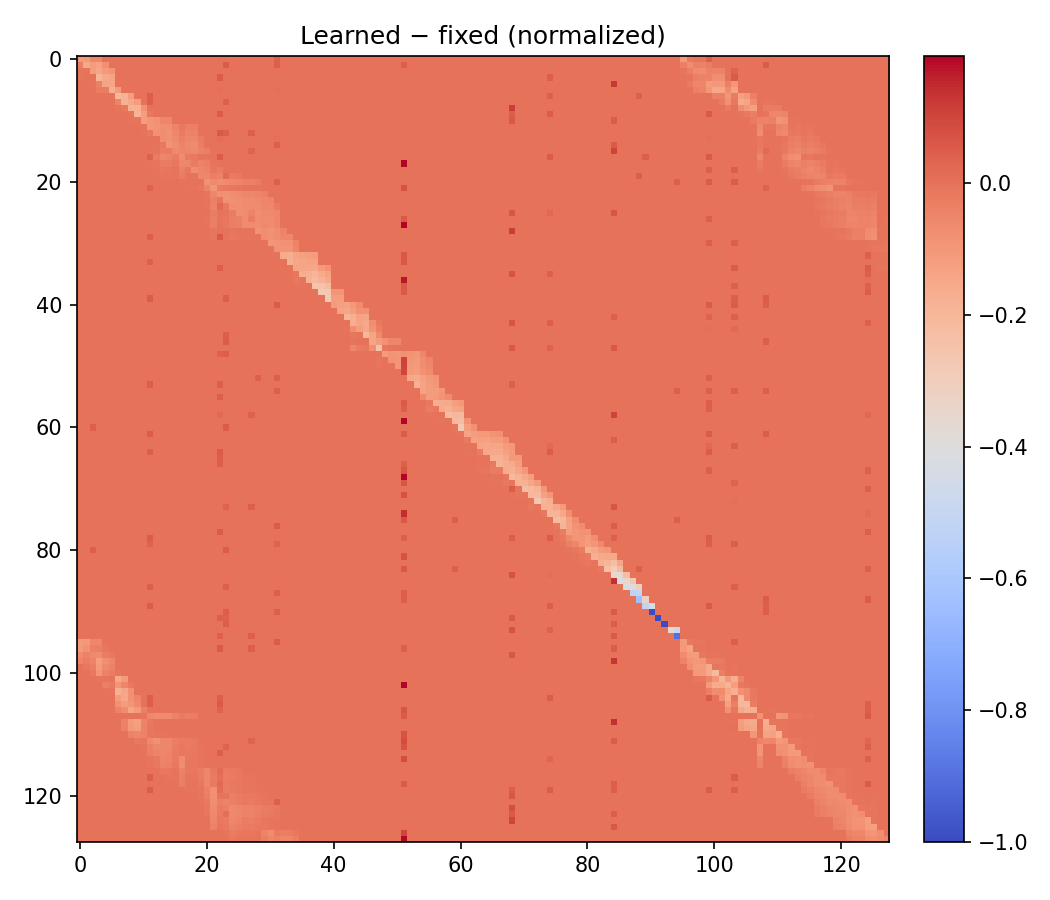
\includegraphics[width=0.32\linewidth]{../figures/q7/stgnn_hybrid_difference.png}
  \caption{Hybrid run: learned component, $\hat{A}$, and difference (crop).}
  \label{fig:q7-diff}
\end{figure}

\subsection{Quantitative alignment with $A$}

Table~\ref{tab:graph-analysis} summarizes \texttt{outputs/graph\_analysis.json} (top-$k=20$ as in training).

\begin{table}[t]
  \centering
  \caption{Learned adjacency vs.\ road-network $A$.}
  \label{tab:graph-analysis}
  \begin{tabular}{lrrr}
    \toprule
    Run & Row entropy & Corr.\ on $A_{ij}>0$ & Top-$k$ overlap / $k$ \\
    \midrule
    stgnn\_adaptive & 2.36 & 0.043 & 0.054 \\
    stgnn\_hybrid & 2.19 & $-0.006$ & 0.033 \\
    \bottomrule
  \end{tabular}
\end{table}

\paragraph{Low overlap with the road graph.}
Mean top-$k$ overlap fraction $|{\mathrm{TopK}_i\cap\mathcal{N}(i)}|/k$ is only $\approx 0.05$ (adaptive) and $\approx 0.03$ (hybrid)---not Jaccard.
For most nodes, the strongest learned edges point \emph{off} the physical adjacency---parallel corridors, distant sensors with correlated patterns, or other statistical shortcuts.
Correlation on pairs where $A_{ij}>0$ is near zero, so even when an edge exists on the map, its learned weight barely tracks the fixed distance weight.

Row entropy $\approx 2.2$--$2.4$ indicates messages spread across many receivers after top-$k$ pruning, rather than collapsing to a single neighbour.
Together with Q6, the picture is clear: the learner \textbf{diverges from $\hat{A}$} and still \textbf{underperforms temporal-only}.
Useful spatial coupling for this task is either already implicit in per-sensor temporal features or not well captured by one shallow GCN step with the adjacencies we tried.
Fixed $\hat{A}$ is the worst choice because it locks in that mismatch; adaptive learning partially repairs it but cannot beat ignoring the graph altogether on this benchmark.

\paragraph{Critical discussion.}
(1) Low forecasting error on an adaptive matrix does \emph{not} mean it rediscovered the road map---predictive edges need not be physical.
(2) Hybrid did \emph{not} outperform adaptive here; the road prior hurt more than it helped.
(3) A static $A$ cannot track rush hours, incidents, or weekend patterns.

\subsection{Pipeline summary}

\begin{itemize}
  \item Graph: $|V|=716$, $A$ from LargeST SD submatrix; message passing uses $\hat{A}$, $A_{\mathrm{adaptive}}$, or hybrid mix.
  \item Time: 15-minute flow, 2020 train / 2021 Q1 val / 2021 Q2--Q4 test; windows $T_{\mathrm{in}}=8$, $H=4$.
  \item Model: 2$\times$ Conv1d temporal encoder ($d=32$), one $\mathrm{ReLU}(A_{\mathrm{msg}} Z W_g)$ layer, linear head; baseline omits the graph layer.
  \item Training: Adam $10^{-3}$, MAE loss, 20 epochs, seed 42.
\end{itemize}

Full reproduction steps are documented in \texttt{scripts/REPRODUCE.md} on the project GitHub.